% Synthetic fixture: a miniature diagram through the node-shape
% subset — circle and rectangle outlines with draw/fill/dashed/thick and
% declared minimums, style bundles, math node bodies (one in a math
% alphabet, as an edge label), transform shape. Invented content and design.
\documentclass{article}

\fonts{ dir = "fonts", body = "Source Serif Pro" }

\begin{document}

\section{Shaped nodes}

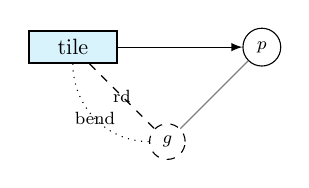
\begin{tikzpicture}[
  scale=0.8, transform shape,
  dot/.style={draw, circle, inner sep=2pt, minimum size=6mm, font=\footnotesize},
  ghost/.style={dashed, draw, circle, font=\footnotesize, minimum size=5mm},
  tile/.style={rectangle, draw, thick, fill=cyan!15, minimum width=14mm, minimum height=5mm}
]
  \node[tile]  (t) at (0, 0) {tile};
  \node[dot]   (p) at (3, 0) {$p$};
  \node[ghost] (g) at (1.5, -1.5) {$g$};
  \draw[-latex] (t) -- (p);
  \draw[gray] (p) -- (g);
  \draw[dashed] (t) -- node[font=\footnotesize] {$\mathrm{rd}$} (g);
  \draw[dotted] (t) to[out=270,in=180] node[font=\footnotesize] {bend} (g);
\end{tikzpicture}

\end{document}
